\begin{lpu}{\texttt{scikit-learn}: Unser Werkzeugkasten fürs ML}
\label{sec:skit}

In diesem Kapitel lernen Sie nun endlich, wie Sie ML-Algorithmen nicht von Hand, sondern mithilfe von python berechnen und verwenden können. Dazu verwenden wir die Bibliothek \texttt{scikit-learn}. Dies ist eine weitverbreitete und stabile Bibliothek für maschinelles Lernen in, die seit 2007 kontinuierlich weiterentwickelt wird und unter einer \textit{open-source}-Lizenz steht.

Ein zentraler Vorteil von \texttt{scikit-learn} besteht darin, dass viele unterschiedliche ML-Algorithmen (z.B. lineare Regression, \textit{k-means}, Entscheidungsbäume; aber auch weitere) über eine einheitliche Programmierschnittstelle verfügbar sind. Das bedeutet: Wenn Sie ein Modell trainiert haben, können Sie unabhängig vom gewählten Algorithmus mit denselben Befehlen Vorhersagen treffen. Diese Modelle werden in \texttt{scikit-learn} als sogenannte \textit{estimators} (Abschätzer) bezeichnet.

\vspace{0.5em}
\textbf{Typische Anwendungsgebiete von \texttt{scikit-learn}:}
\begin{itemize}
  \item Klassifikation (z. B. Vorhersage von Kategorien wie ``spam'' oder ``ham'')
  \item Regression (z. B. Vorhersage eines numerischen Werts)
  \item Ballung (\textit{clustering}), also das Gruppieren ähnlicher Daten ohne Vorwissen
\end{itemize}

\vspace{0.5em}
\texttt{scikit-learn} eignet sich besonders für klassische Machine-Learning-Verfahren auf einem einzigen Rechner. Es bietet darüber hinaus hilfreiche Funktionen für:
\begin{itemize}
  \item das automatische Aufteilen Ihres Datensatzes in Trainings- und Testdaten
  \item die Normierung (Skalierung) von Daten
  \item das Speichern und Laden von Modellen
\end{itemize}

Für anspruchsvollere ML-Verfahren, insbesondere im Bereich des \textit{deep learning}, sind andere Bibliotheken wie \texttt{PyTorch} oder \texttt{TensorFlow} mit \texttt{Keras} besser geeignet. Diese bieten spezialisierte Funktionen zum Aufbau neuronaler Netzwerke und nutzen Grafikprozessoren (GPUs), um komplexe Berechnungen effizient auszuführen. Die Einstiegshürde ist dort jedoch deutlich höher. Wir verwenden in dieser Unterrichtseinheit deshalb ausschliesslich \texttt{scikit-learn}, da es durch seine klare Struktur, einheitliche API und einfache Bedienbarkeit besonders geeignet für den Einstieg ist.

\vspace{1em}
\begin{center}
  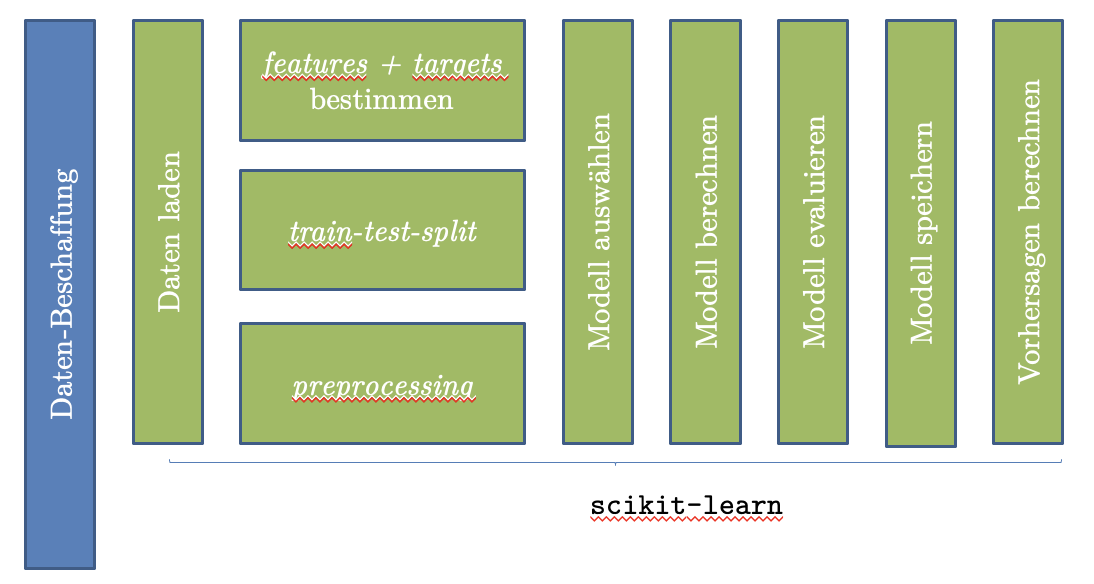
\includegraphics[width=0.9\linewidth]{pipeline.png}
\end{center}

Die obige Abbildung zeigt den typischen Arbeitsablauf bei einem ML-Projekt mit \texttt{scikit-learn}:

\begin{enumerate}
  \item \textbf{Daten-Beschaffung:} Die Daten müssen zunächst aus einer Quelle (z. B. CSV-Datei, Datenbank, API) bezogen werden. Dabei kann Ihnen \texttt{scikit-learn} für gewöhnlich nicht helfen, ausser Sie greifen auf einer der mitgelieferten Datensätzen zur Demonstration zurück (wie wir es gleich tun werden).
  \item \textbf{Daten laden:} Anschliessend werden die Daten in \texttt{python} eingelesen.
  \item \textbf{\textit{features} und \textit{targets} bestimmen:} Es wird festgelegt, welcher Teil der Daten als Eingabe (features, meist \texttt{X}) und welche als Zielvariable (target, meist \texttt{y}) verwendet werden.
  \item \textbf{\textit{train-test-split}:} Der Datensatz wird aufgeteilt in Trainings- und Testdaten, um eine faire Evaluierung zu ermöglichen.
  \item \textbf{\textit{preprocessing}:} Die Daten werden vorbereitet (z. B. skaliert), um für die Algorithmen geeignet zu sein.
  \item \textbf{Modell auswählen:} Es wird ein passender Algorithmus gewählt (z. B. Entscheidungsbaum).
  \item \textbf{Modell berechnen:} Das Modell wird mit den Trainingsdaten trainiert (Methode: \texttt{.fit()}).
  \item \textbf{Modell evaluieren:} Das Modell wird mit den Testdaten getestet, z. B. über \texttt{.score()} oder \texttt{confusion\_matrix()}.
  \item \textbf{Modell speichern:} Gute Modelle können gespeichert werden, z. B. mit \texttt{joblib.dump()}.
  \item \textbf{Vorhersagen berechnen:} Für neue, unbekannte Daten können Vorhersagen getroffen werden (\texttt{.predict()}).
\end{enumerate}

Wir gehen nun auf die einzelnen Schritte genauer ein!

\begin{hinweis}
    Da wir uns nun in die Welt von Python begeben, ist es vielleicht einfacher, wenn Sie dieser LPU mit dem beiliegenden Notizbuch \texttt{files/LA\_1650} folgen. Dort können Sie die Befehle, welche in diesem Kapitel aufgelistet sind, direkt ausprobieren.
\end{hinweis}

Bevor Sie überhaupt etwas mit \texttt{scikit-learn} tun können, müssen Sie es zunächst installieren. Dafür verwenden Sie in Ihrem Terminal folgenden Befehl:

\begin{lstlisting}[language=Bash]
pip install sklearn
\end{lstlisting}

Falls Sie im Notizbuch sind, können Sie dort einfach die Zelle \texttt{!pip install sklearn} ausführen.


\subsubsection*{Iris-Datensatz}
Ein typischer Einstieg in die ML-Welt erfolgt mit dem berühmten Iris-Datensatz, bei dem für verschiedene Iris-Blumenarten L"angen von Bl"uten- und Kelchbl"attern gemessen wurden. Ziel ist es, anhand dieser Merkmale (\textit{features}) die Blumenart (\textit{target}) vorherzusagen. Dieses Beispiel gilt als das \texttt{Hello World} in der Welt des maschinellen Lernens!

\begin{center}
  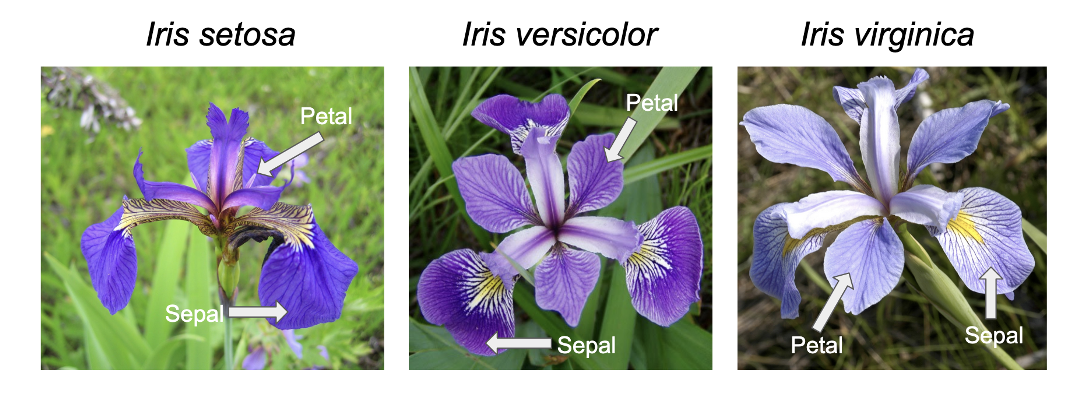
\includegraphics[width=0.9\linewidth]{iris.png}
\end{center}

Um diesen Datensatz einfach zu importieren, verwenden Sie folgenden Befehl:

\begin{lstlisting}[language=Python]
from sklearn.datasets import load_iris
iris = load_iris(as_frame=True)
\end{lstlisting}

Der Parameter \texttt{as\_frame} erlaubt uns, den Datensatz als \texttt{pandas DataFrame}-Objekt zu laden. Der Umgang mit solchen Objekten ist — wie Sie gleich sehen werden — sehr intuitiv und erlaubt es Ihnen, die Daten wie eine Tabelle zu behandeln.

\subsubsection*{\textit{target} und \textit{features}}
In diesem Schritt entscheiden Sie, was genau Sie vorhersagen möchten (das nennt man \textit{target} oder auch \textit{Zielvariable}), und welche Daten dafür als Grundlage dienen sollen (das sind die \textit{features}). Das variiert je nach Datensatz und Ihrem Interesse. Mit demselben Datensatz können Sie ganz unterschiedliche Modelle produzieren, je nachdem, wie Sie das \textit{target} setzen.



\begin{table}[h!]
\centering
\begin{tabular}{|c|c|c|c|c|c|}
\hline
\textbf{age} & \textbf{sex} & \textbf{bmi} & \textbf{smoker} & \textbf{region} & \textbf{health insurance charges} \\
\hline
19 & \male & 27.9  & yes & southwest & 16884 \\
18 & \female & 33.77 & no  & southeast & 1725  \\
28 & \female & 33.0  & no  & southeast & 4449  \\
33 & \female & 22.0  & no  & northwest & 8240  \\
\hline
\end{tabular}
\caption{Beispieldatensatz zu Gesundheitskosten und personenbezogenen Merkmalen}
\end{table}

Aus den Daten in der Tabelle oben können Sie bspw. ein Modell erstellen, was die Krankenkasse-Prämie berechnet basierend auf Alter, BMI und Tabakkonsum. In dem Fall wäre die Prämie das \textit{target} (nachfolgend \colorbox{lightgray}{\textcolor{targetred}{rot}}) und Alter, BMI und Tabakkonsum die \textit{features} (nachfolgend \colorbox{lightgray}{\textcolor{featuregreen}{grün}}). 

\begin{table}[h!]
\centering
\rowcolors{2}{white}{gray!10}
\begin{tabular}{|>{\columncolor{featuregreen}}c|
                c|
                >{\columncolor{featuregreen}}c|
                >{\columncolor{featuregreen}}c|
                c|
                >{\columncolor{targetred}}c|}
\hline
\textbf{age} & \textbf{sex} & \textbf{bmi} & \textbf{smoker} & \textbf{region} & \textbf{health insurance charges} \\
\hline
19 & ♀ & 27.9  & yes & southwest & 16884 \\
18 & ♂ & 33.77 & no  & southeast & 1725  \\
28 & ♂ & 33.0  & no  & southeast & 4449  \\
33 & ♂ & 22.0  & no  & northwest & 8240  \\
\hline
\end{tabular}
\caption{Variante 1: Vorhersage der Krankenkassenprämie aus Alter, BMI und Rauchverhalten}
\end{table}



Aber Sie könnten auch versuchen, den BMI vorherzusagen (\textit{target}) ausgehend auf Alter, Wohnort und Geschlecht (\textit{features}).

\begin{table}[h!]
\centering
\rowcolors{2}{white}{gray!10}
\begin{tabular}{|>{\columncolor{featuregreen}}c|
                >{\columncolor{featuregreen}}c|
                >{\columncolor{targetred}}c|
                c|
                >{\columncolor{featuregreen}}c|
                c|}
\hline
\textbf{age} & \textbf{sex} & \textbf{bmi} & \textbf{smoker} & \textbf{region} & \textbf{health insurance charges} \\
\hline
19 & ♀ & 27.9  & yes & southwest & 16884 \\
18 & ♂ & 33.77 & no  & southeast & 1725  \\
28 & ♂ & 33.0  & no  & southeast & 4449  \\
33 & ♂ & 22.0  & no  & northwest & 8240  \\
\hline
\end{tabular}
\caption{Variante 2: Vorhersage des BMI aus Alter, Geschlecht und Region}
\end{table}




Im Falle unseres Iris-Datensatzes wird uns das Leben hier aber sehr einfach gemacht: Im Datensatz sind die Kolonnen bereits mit \texttt{.data} und \texttt{.target} benannt. \texttt{.data} enthält die Längen der Blüten, und \texttt{.target} die Kategorisierung (\texttt{0} für \textit{Iris setosa}, \texttt{1} für \textit{Iris versicolor} und \texttt{2} für \textit{Iris virginica}). Wir müssen also diese Kolonnen lediglich in unterschiedlichen Variablen speichern, um diese Unterteilung in \textit{target} und \textit{features} zu machen:

\begin{lstlisting}[language=Python]
X = iris.data
y = iris.target
\end{lstlisting}

Wir hätten \texttt{X} und \texttt{y} auch \texttt{features} und \texttt{target} nennen können; aber diese Nomenklatur hat sich für ML-Code eingebürgert. Im Notizbuch können Sie sich mit \texttt{X[:10], y[:10]} auch anzeigen lassen, was nun in diesen Variablen gespeichert wurde.

\begin{theorie}
    Im maschinellen Lernen bezeichnet \textit{target} die \textit{Zielvariable}, also das, was ein Modell vorhersagen können soll. Im Code wird diese üblicherweise mit \texttt{y} bezeichnet.

    \textit{features} nennen wir die Daten, die wir zur Berechnung des \textit{target}s heranziehen. Als Variable im Code heissen diese \texttt{X}.
\end{theorie}

\subsubsection*{\textit{train-test split}}

Wenn ein Modell trainiert wird, besteht die Gefahr, dass es die vorhandenen Daten zu gut lernt – man spricht dann von einer ``Überanpassung'' (\textit{overfitting}). Ein solches Modell funktioniert zwar sehr gut auf den Daten, die es bereits kennt, aber schlecht auf neuen, unbekannten Daten. Das ist ein bisschen wie ``auswendig lernen, ohne zu verstehen''.

\begin{aufgabe}{1: \textit{overfitting} oder echtes Verständnis?}

Stellen Sie sich vor, Ihre Sitznachbarin möchte unbedingt eine gute Note in der nächsten Biologieprüfung. Sie weiss, dass die Lehrperson letztes Jahr eine Prüfung mit 20 Fragen gestellt hat – und dass der genaue Wortlaut dieser alten Prüfung noch im Umlauf ist.

Sie entscheidet sich, diese alte Prüfung auswendig zu lernen – inklusive der genauen Fragestellung und aller Antworten. Am Prüfungstag stellt sich jedoch heraus: Die Lehrperson hat die Fragen leicht verändert.

Hat Ihre Sitznachbarin ``gelernt'' oder nur ``auswendig gelernt''? Was wird das Prüfungsergebnis vermutlich zeigen? Und was hat das mit maschinellem Lernen zu tun?

\begin{itemize}
  \item Erklären Sie den Begriff \textit{overfitting} mit eigenen Worten anhand dieses Beispiels.
  \item Überlegen Sie, wie man das beim Trainieren eines ML-Modells vermeiden könnte.
\end{itemize}
\end{aufgabe}

Analog müssen wir also auch bei unseren Modellen mit Daten, die das Modell noch nicht gesehen hat, aber für die wir als ``Lehrer'' die korrekte Antwort kennen, die Qualität unseres Modells testen, bevor wir es in die freie Wildbahn entlassen.

Aus diesem Grund werden unsere Daten eingeteilt in einen \textit{train} und einen \textit{test}-Teil. Die \textit{train}-Daten (wie \textit{training}, nicht wie das Verkehrsmittel) dienen als Grundlage, um ein Modell zu berechnen; und die Test-Daten werden verwendet, um zu überprüfen, wie gut das Modell für Daten ist, die es noch nicht kennt.

Der \textit{train}- und \textit{test}-Teil sind beide jeweils wie vorhin unterteilt in \texttt{X} und \texttt{y}, wie die nachfolgende Abbildung veranschaulicht:

\vspace{1em}
\begin{center}
  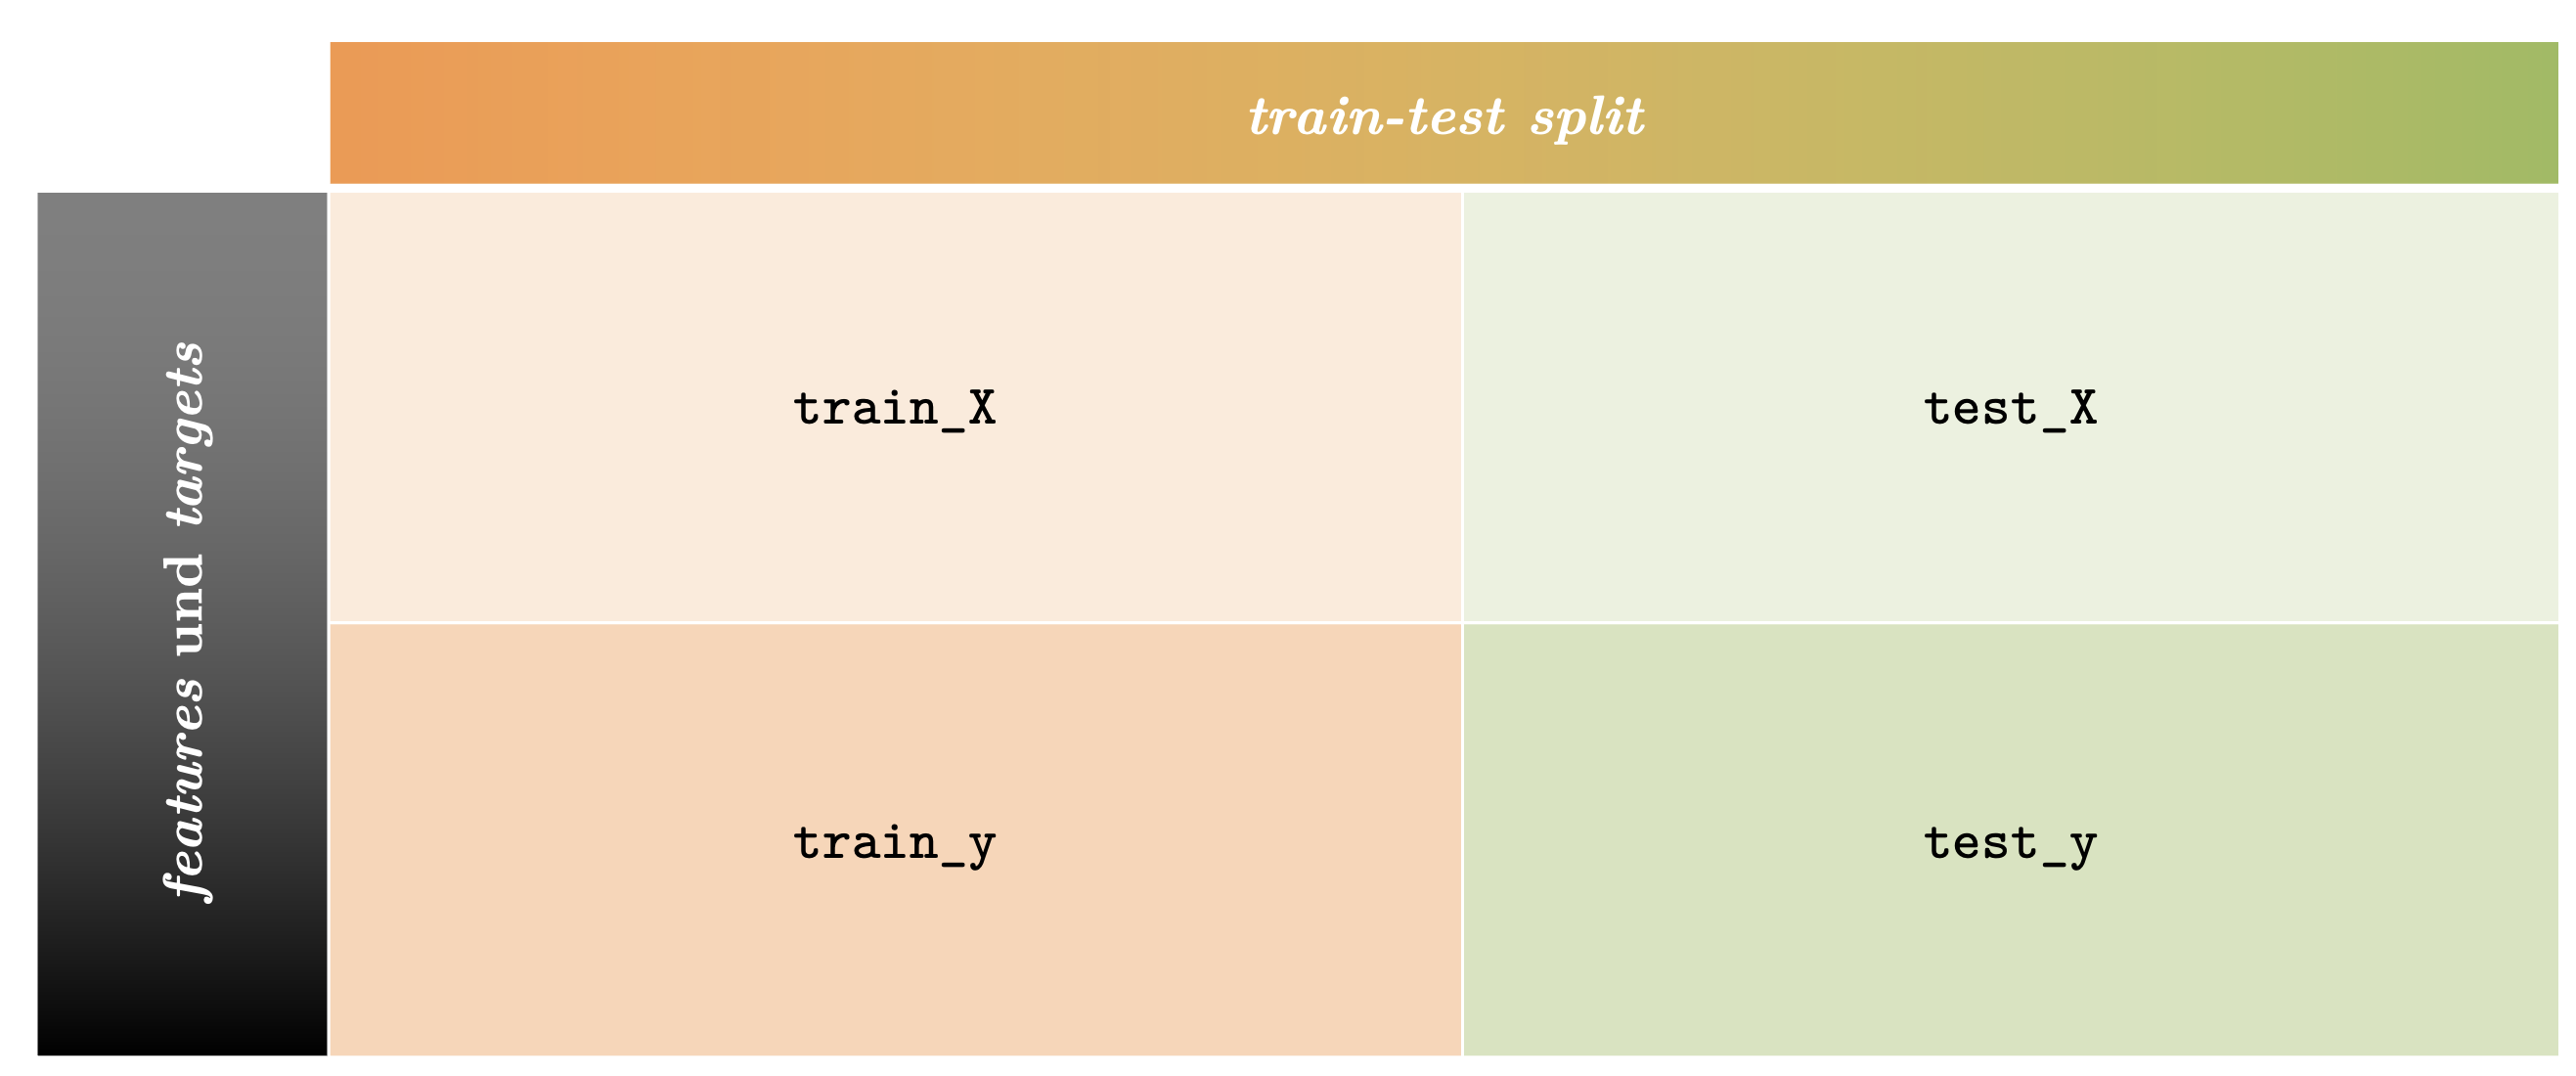
\includegraphics[width=0.9\linewidth]{testtrain.png}
\end{center}

Die meisten fortgeschrittenen Algorithmen werden \textit{iterativ}, das heisst, in mehreren Runden, ausgehend von den \textit{train}-Daten berechnet. Der Algorithmus bekommt also die Test-Daten hier nicht zu Gesicht. Nach jeder Runde wird das Modell getestet, indem die Vorhersage des Modells ausgehend von den \texttt{X}-Werten der Test-Daten mit den tatsächlichen \texttt{y}-Werten der Test-Daten verglichen wird. So kann im Vorfeld berechnet werden, wie gut das Modell für neue Daten Vorhersagen treffen wird.




\begin{figure}[h!]
\centering
\begin{subfigure}[t]{0.45\textwidth}
  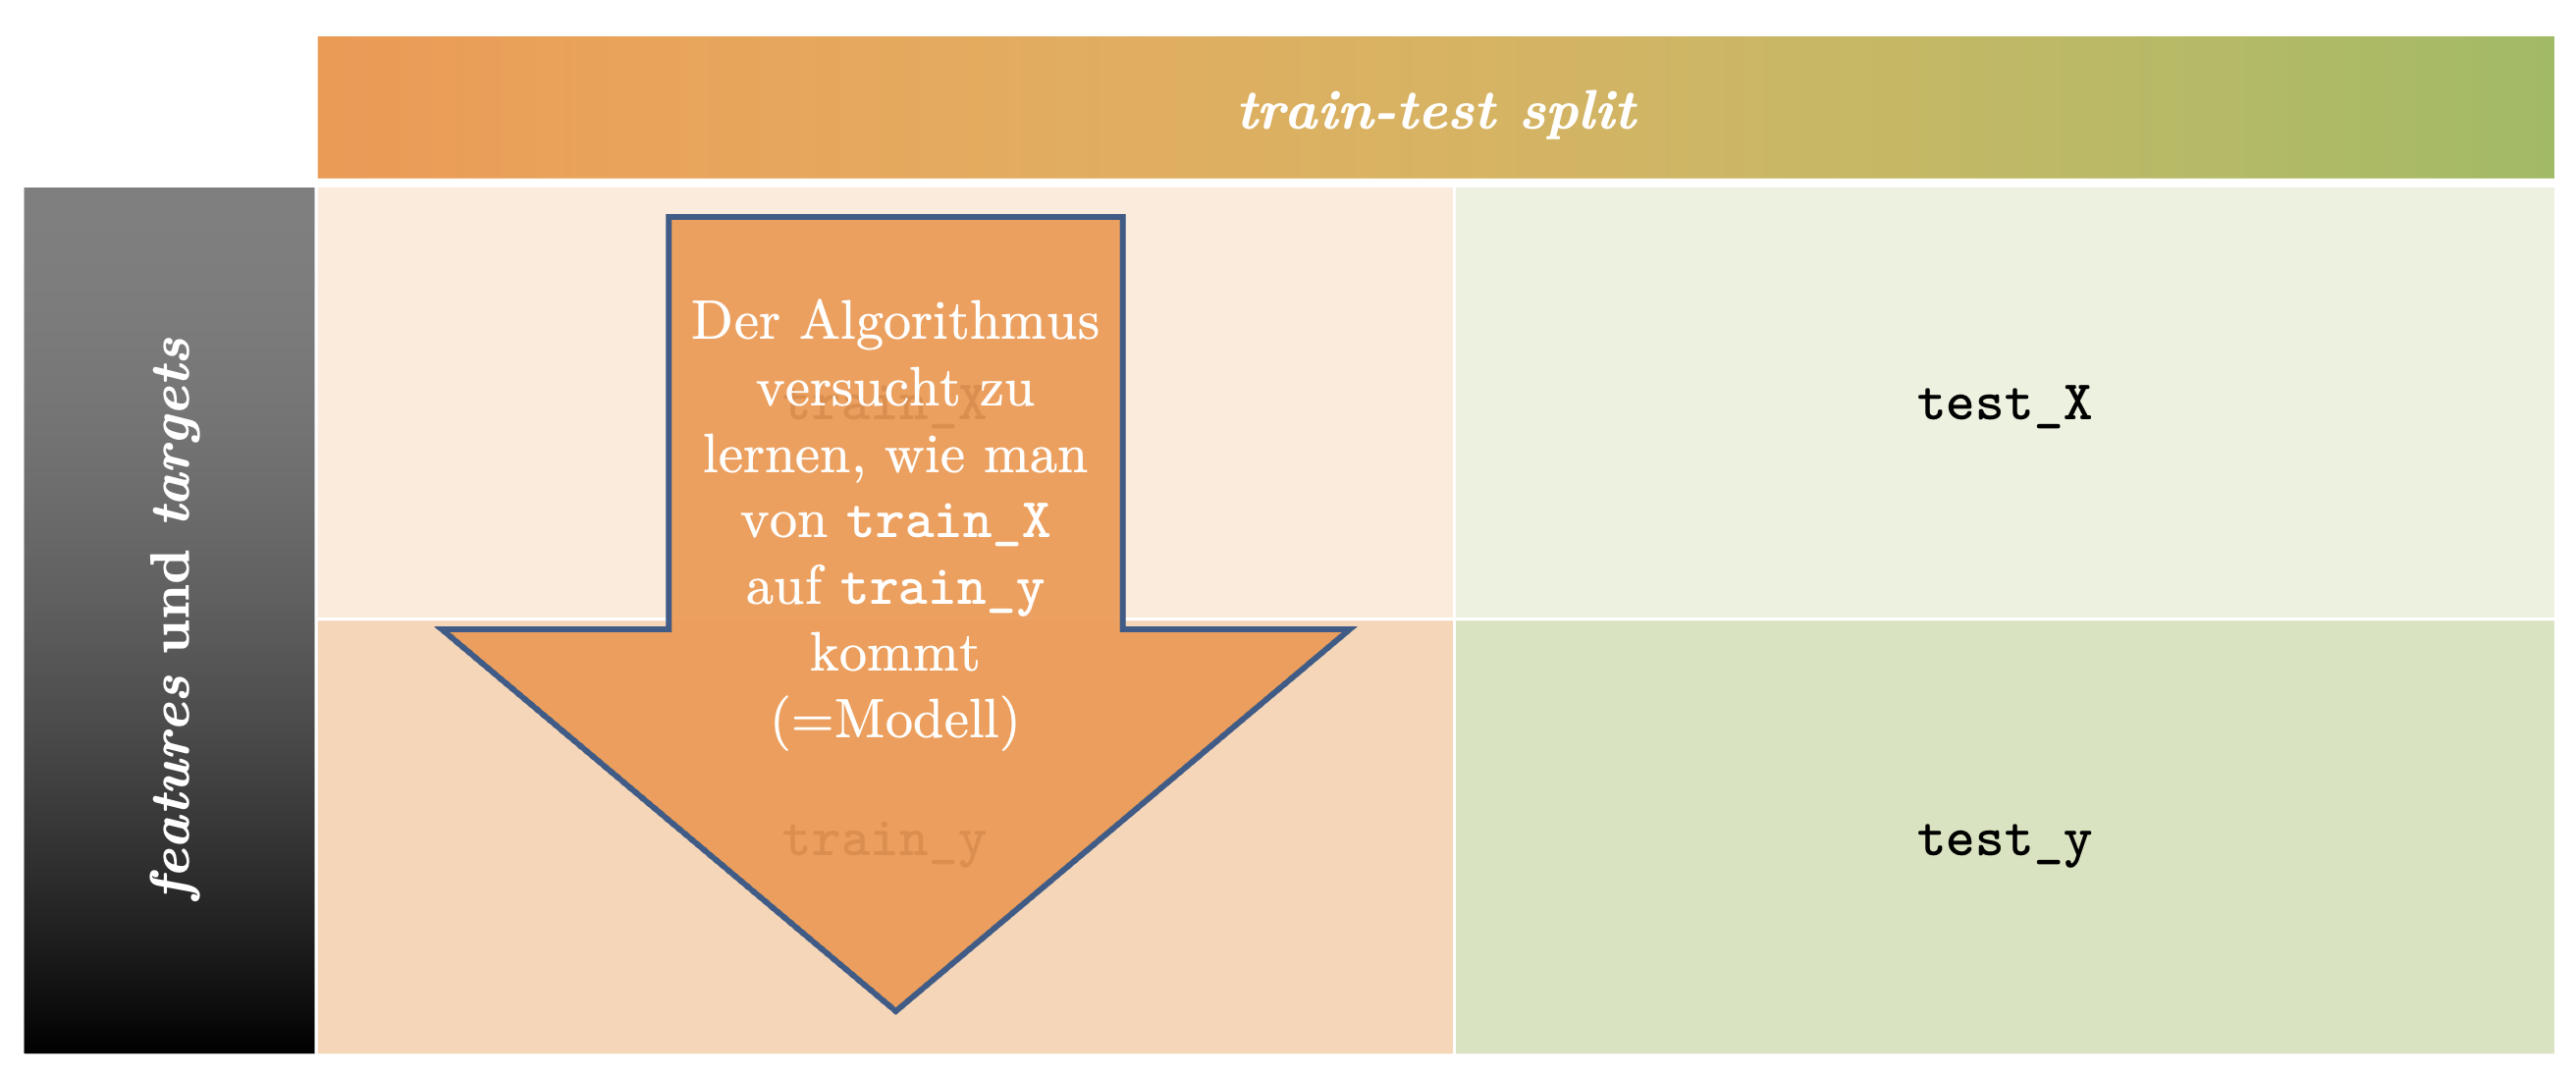
\includegraphics[width=\linewidth, valign=t]{testtrain_1.png}
  \caption{Schritt 1}
\end{subfigure}
\hfill
\begin{subfigure}[t]{0.45\textwidth}
  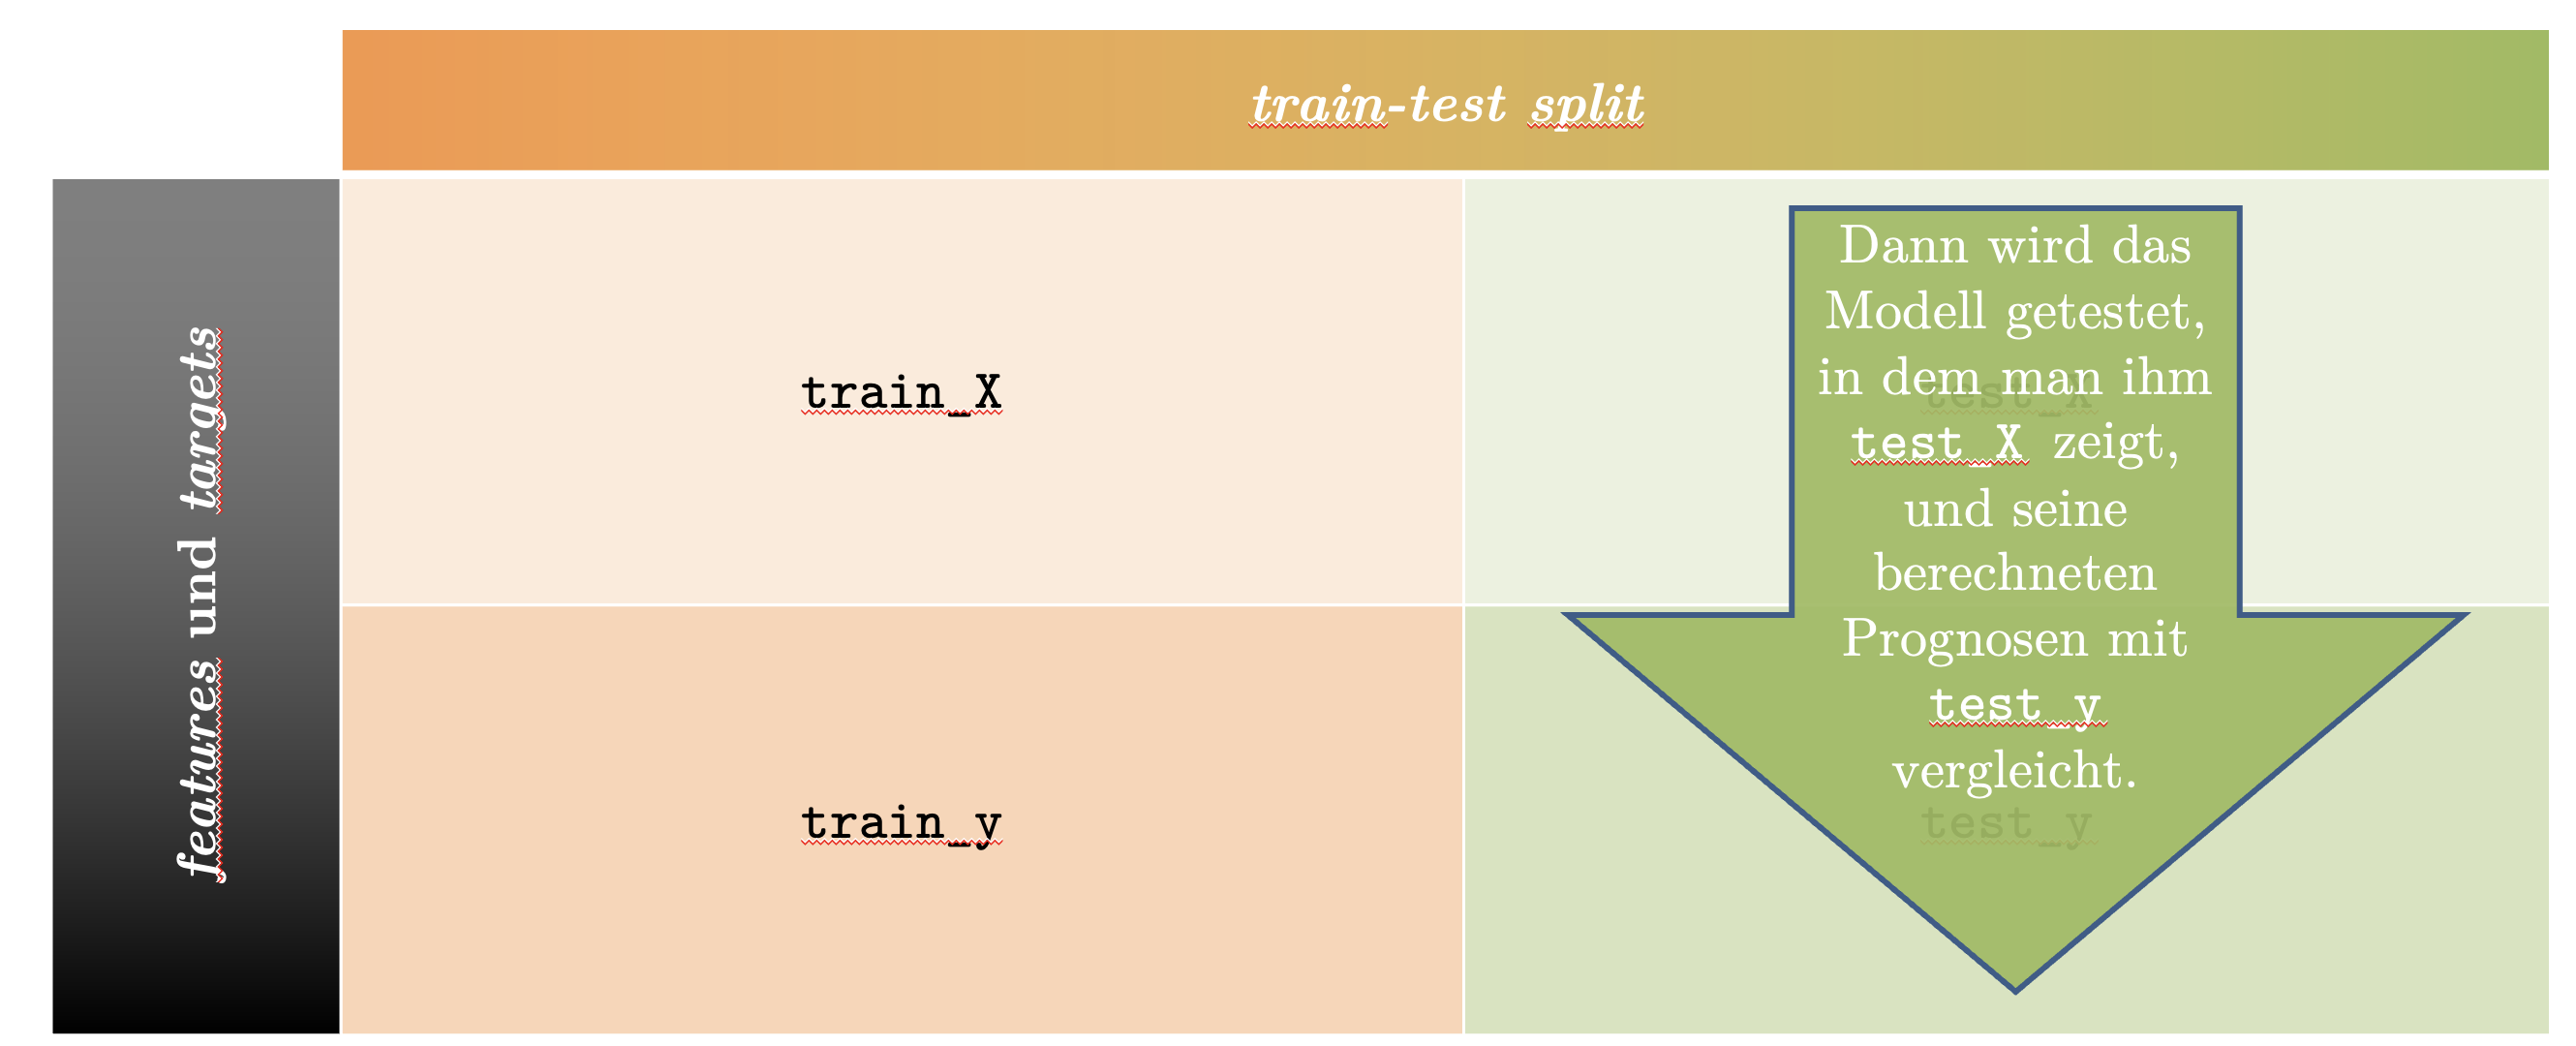
\includegraphics[width=\linewidth, valign=t]{testtrain_2.png}
  \caption{Schritt 2}
\end{subfigure}
\vspace{1em}
\begin{subfigure}[t]{0.45\textwidth}
  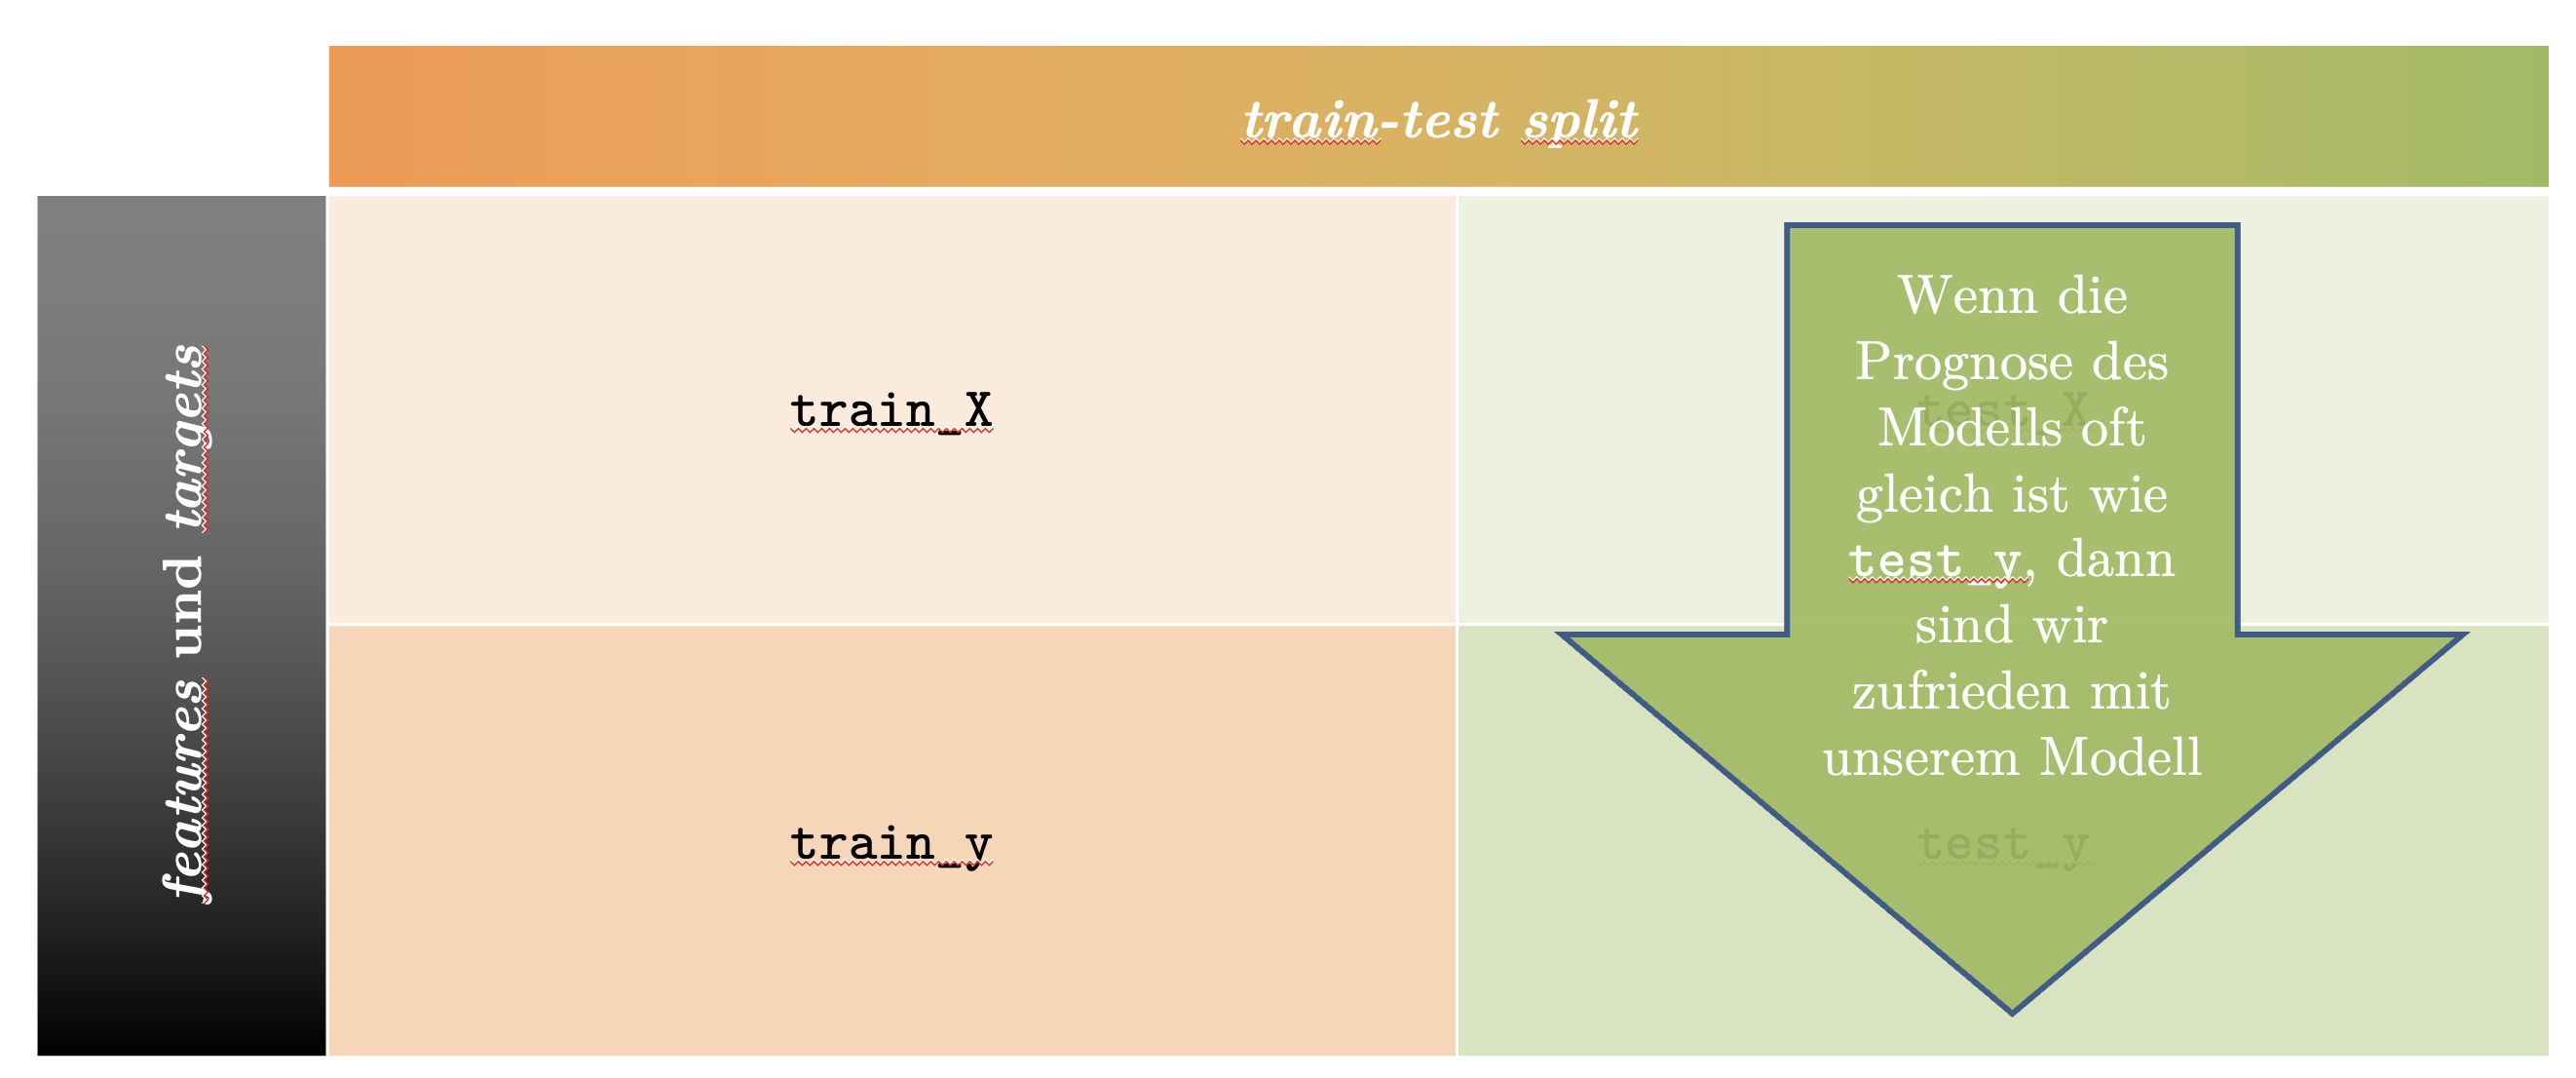
\includegraphics[width=\linewidth, valign=t]{testtrain_3.png}
  \caption{Schritt 3}
\end{subfigure}
\hfill
\begin{subfigure}[t]{0.45\textwidth}
  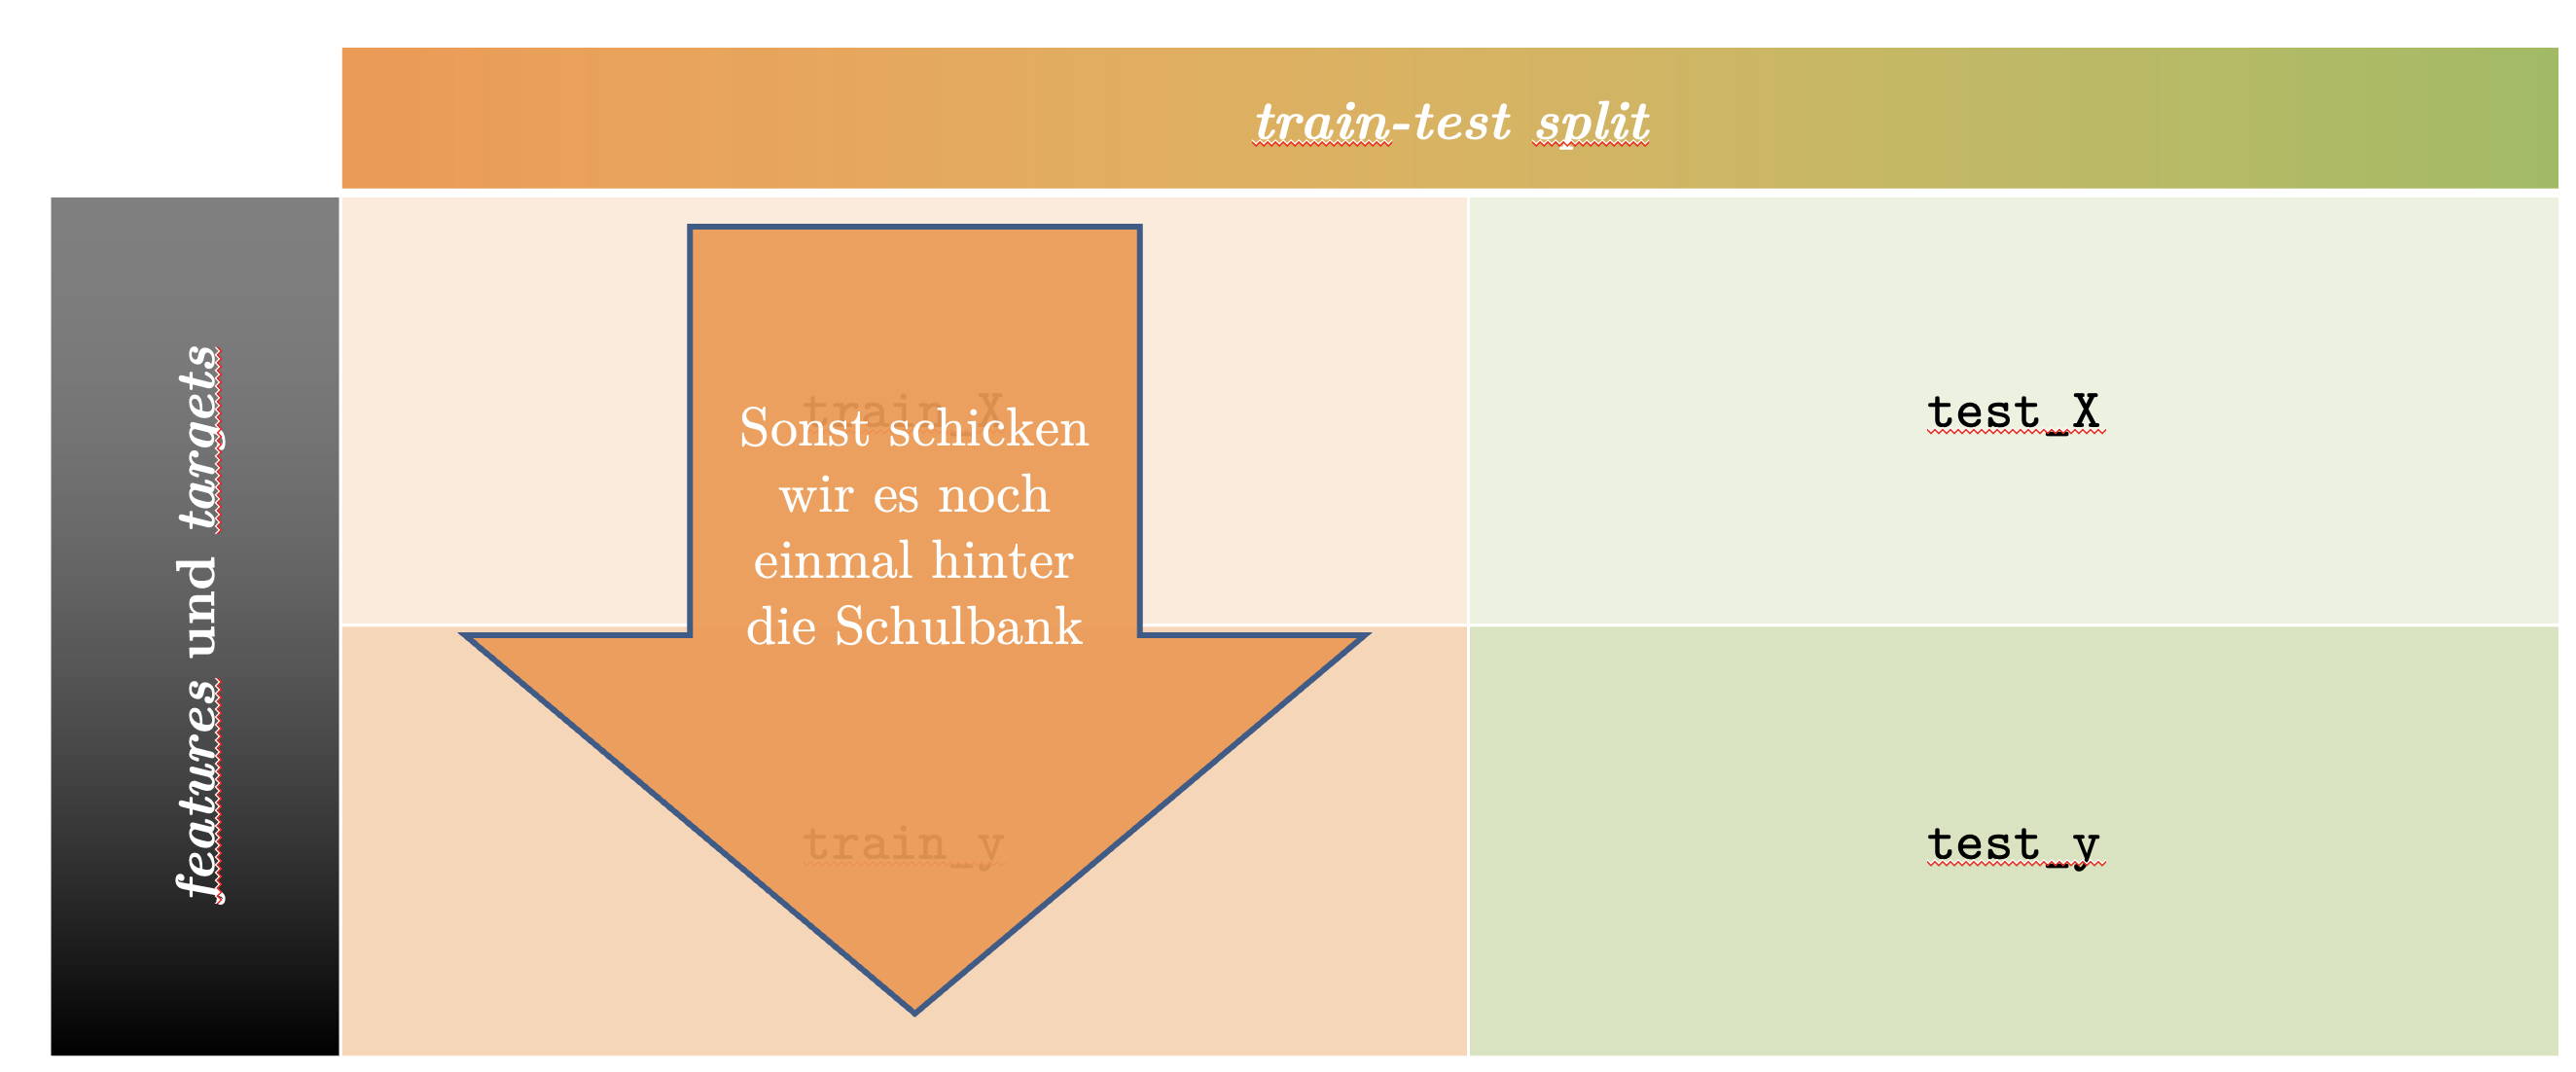
\includegraphics[width=\linewidth, valign=t]{testtrain_4.png}
  \caption{Schritt 4}
\end{subfigure}
\end{figure}






Beim maschinellen Lernen wird der Datensatz in der Regel wie folgt in diese zwei Teile aufgeteilt:
\begin{itemize}
  \item Trainingsdaten: etwa 70–90\,\%
  \item Testdaten: etwa 10–30\,\%
\end{itemize}

Ein Modell benötigt möglichst viele Beispiele, um verlässliche Muster zu erkennen. Wenn zu wenig Daten für das Training verwendet werden, lernt das Modell nicht genug – insbesondere bei kleinen Datensätzen. Ein 50:50-Split ist darum meist ineffizient.

\begin{itemize}
  \item {80\,\% / 20\,\% ist ein verbreiteter Kompromiss: genügend Trainingsdaten, aber auch ausreichend Testdaten für eine seriöse Evaluation.
  \item Bei sehr grossen Datensätzen (z.\,B. >100\,000 Beispiele) sind auch 90\,\% / 10\,\% sinnvoll, da bereits 10\,\% eine grosse Testmenge darstellen.
  \item Bei kleinen Datensätzen wird manchmal eine 70\,\% / 30\,\%-Aufteilung verwendet, um mehr Testbeispiele zu erhalten. (Alternativ kann \textit{cross validation} eingesetzt werden, aber diese sprengt den Rahmen dieser Unterrichtseinheit. Interessierte SuS können \href{https://machinelearningmastery.com/k-fold-cross-validation}{hier}\footnote{\href{https://machinelearningmastery.com/k-fold-cross-validation}{\url{machinelearningmastery.com/k-fold-cross-validation}}} beispielsweise mehr erfahren.)
\end{itemize}

\begin{theorie}

Beim maschinellen Lernen wird der verfügbare Datensatz in zwei Teile aufgeteilt: 
\textbf{Trainingsdaten} (\textit{train set}) und \textbf{Testdaten} (\textit{test set}). Das Modell wird ausschliesslich mit den Trainingsdaten ``gelernt'' – die Testdaten dienen dazu, die Leistung des Modells auf \textit{neuen, unbekannten Daten} zu überprüfen. Nur so kann man feststellen, ob das Modell wirklich generalisiert oder lediglich auswendig gelernt hat (\textit{overfitting}).
\end{theorie}

In \texttt{scikit-learn} ist auch dieser Schritt sehr einfach: Mit dem folgenden Befehl passiert diese Einteilung automatisch:




\begin{lstlisting}[language=Python]
from sklearn.model_selection import train_test_split

X_train, X_test, y_train, y_test = train_test_split(
   X, y, test_size = 0.3, random_state = 42
)
\end{lstlisting}


Die Bedeutung der einzelnen Variablen ist:

\begin{itemize}
  \item \texttt{X}: Variable mit den \textit{features} (z. B. Länge der Blüten, oder Wohnort, Rauchverhalten etc. im Krankenkassen-Beispiel)
  \item \texttt{y}: Variable mit dem \textit{target} (z. B. Iris-Art oder Versicherungskosten)

  \item \texttt{X\_train}: Features der Trainingsdaten
  \item \texttt{X\_test}: Features der Testdaten
  \item \texttt{y\_train}: Zielwerte der Trainingsdaten
  \item \texttt{y\_test}: Zielwerte der Testdaten
\end{itemize}

\texttt{test\_size = 0.3} bedeutet, dass 30\,\% der Daten für das Testset verwendet werden. Da unser Datensatz so klein ist, ist das hier sinnvoll.
\texttt{random\_state = 42} sorgt dafür, dass die Aufteilung \textit{reproduzierbar} ist: Zwar werden die Daten ``zufällig'' in \textit{test}- und \textit{train}-Teile aufgeteilt, aber immer, wenn jemand \texttt{random\_state = 42} für \textit{diesen} Datensatz verwendet, sieht die Aufteilung gleich aus. Würde jemand \texttt{random\_state = 33} verwenden, hingegen, sähe sie anders aus. Das ist wichtig, wenn Sie Ihre Arbeit reproduzierbar machen möchten.

\subsubsection*{Aufbereitung}

Bevor ein ML-Modell mit den Daten trainiert wird, müssen diese oft vorbereitet werden – man spricht von \textit{preprocessing} (wörtlich Vorverarbeitung). Das Ziel ist es, die Daten in eine Form zu bringen, mit der der Algorithmus effizient und korrekt arbeiten kann.

Eine zentrale Technik, die Sie bereits kennen, ist die \textit{Skalierung}. Numerische Werte wie z. B. Alter oder Einkommen werden auf einen gemeinsamen Zahlenbereich gebracht (z. B. $[0,1]$), damit einzelne Spalten das Modell nicht übermässig beeinflussen.

Darüber hinaus gibt es weitere wichtige Möglichkeiten der Aufbereitung:

\begin{itemize}
  \item \textit{one hot encoding:} Kategorische Merkmale wie ``Region'' oder ``Geschlecht'' werden in Zahlen umgewandelt.
  \item Fehlende Werte behandeln: Leere Zellen (NaN) werden z.B. durch Mittelwerte oder spezielle Marker ersetzt.
  \item Text-Vektorisierung: Texte müssen in Zahlen umgewandelt werden, da viele Modelle nicht gut natürlichen Text verarbeiten können. Das wird oft mittels \textit{embeddings} gemacht, sodass der gesamte Text als ein mathematischer Vektor ausgedrückt werden kann. (Dies nur zur Information; diese Technik geht weit über den Rahmen dieser Unterrichtseinheit hinaus.)
\end{itemize}

\texttt{scikit-learn} stellt für all diese Schritte praktische Funktionen bereit, z.B. \texttt{StandardScaler}, \texttt{OneHotEncoder} oder \texttt{SimpleImputer}.

\begin{aufgabe}{2}
Schauen Sie sich den Iris-Datensatz etwas genauer an (bspw. mit \texttt{X[:10], y[:150]} im Notizbuch):

\begin{enumerate}
    \item Finden Sie in diesem Datensatz das oben erwähnte \textit{one hot encoding} wieder?
    \item Die \texttt{X}-Werte enthalten verschiedene Arten von Messungen (nämlich die Breite und Länge der Blütenblätter und die Länge und Breite des Kelchblatts). Befinden sich diese alle im selben Wertebereich? Würden Sie eine Skalierung hier als sinnvoll erachten?
\end{enumerate}
\end{aufgabe}

Wenn wir unsere Daten aufbereiten müssen, dann macht es uns \texttt{scikit-learn} wieder ungemein einfach:
\begin{lstlisting}[language=Python]
from sklearn import preprocessing
scaler = preprocessing.MinMaxScaler()
X_train_scaled = scaler.fit_transform(X_train)
X_test_scaled = scaler.transform(X_test)
\end{lstlisting}

Damit skalieren wir \texttt{X\_train} und \texttt{X\_test} mit dem \texttt{MinMaxScaler}, der alle Werte auf einen Bereich von \texttt{0} bis \texttt{1} bringt. Es gibt auch andere Algorithmen, welche den Wertebereich bspw. auf $[-1,1]$ skalieren. Weiterhin:

\begin{itemize}
  \item \texttt{fit\_transform(X\_train)}: berechnet Minimum und Maximum auf Basis der Trainingsdaten und wendet die Skalierung direkt an.
  \item \texttt{transform(X\_test)}: verwendet genau dieselben minimalen und maximalen Grenzwerte, um auch die Testdaten korrekt zu skalieren.
\end{itemize}

Die Testdaten dürfen nicht in die Berechnung der Skalierung einfliessen, da sonst ein ausgefuchster Algorithmus daraus Rückschlüsse auf die Testdaten schliessen könnte.


\subsubsection*{Modellauswahl}

In \texttt{scikit-learn} stehen viele verschiedene ML-Modelle zur Verfügung. Doch welches Modell ist das Richtige? Natürlich gibt es verschiedene Algorithmen für verschiedene Probleme (bspw. Entscheidungsbäume für Kategorisierung), aber selbst innerhalb einer Problem-Klasse gibt es viele Algorithmen mit unterschiedlichen Vor- und Nachteilen.

In der Praxis testet man oft mehrere Modelle und vergleicht sie anhand ihrer Leistung auf den Test-Daten. \texttt{scikit-learn} macht diesen Vergleich sehr einfach, weil alle Modelle eine ähnliche API (\texttt{fit()}, \texttt{predict()}, \texttt{score()}) verwenden.

Die nachfolgende Grafik gibt aber eine gute Übersicht, was innerhalb von \texttt{sklearn} möglich ist, und wie Sie eine erste Auswahl treffen können:

\begin{center}
  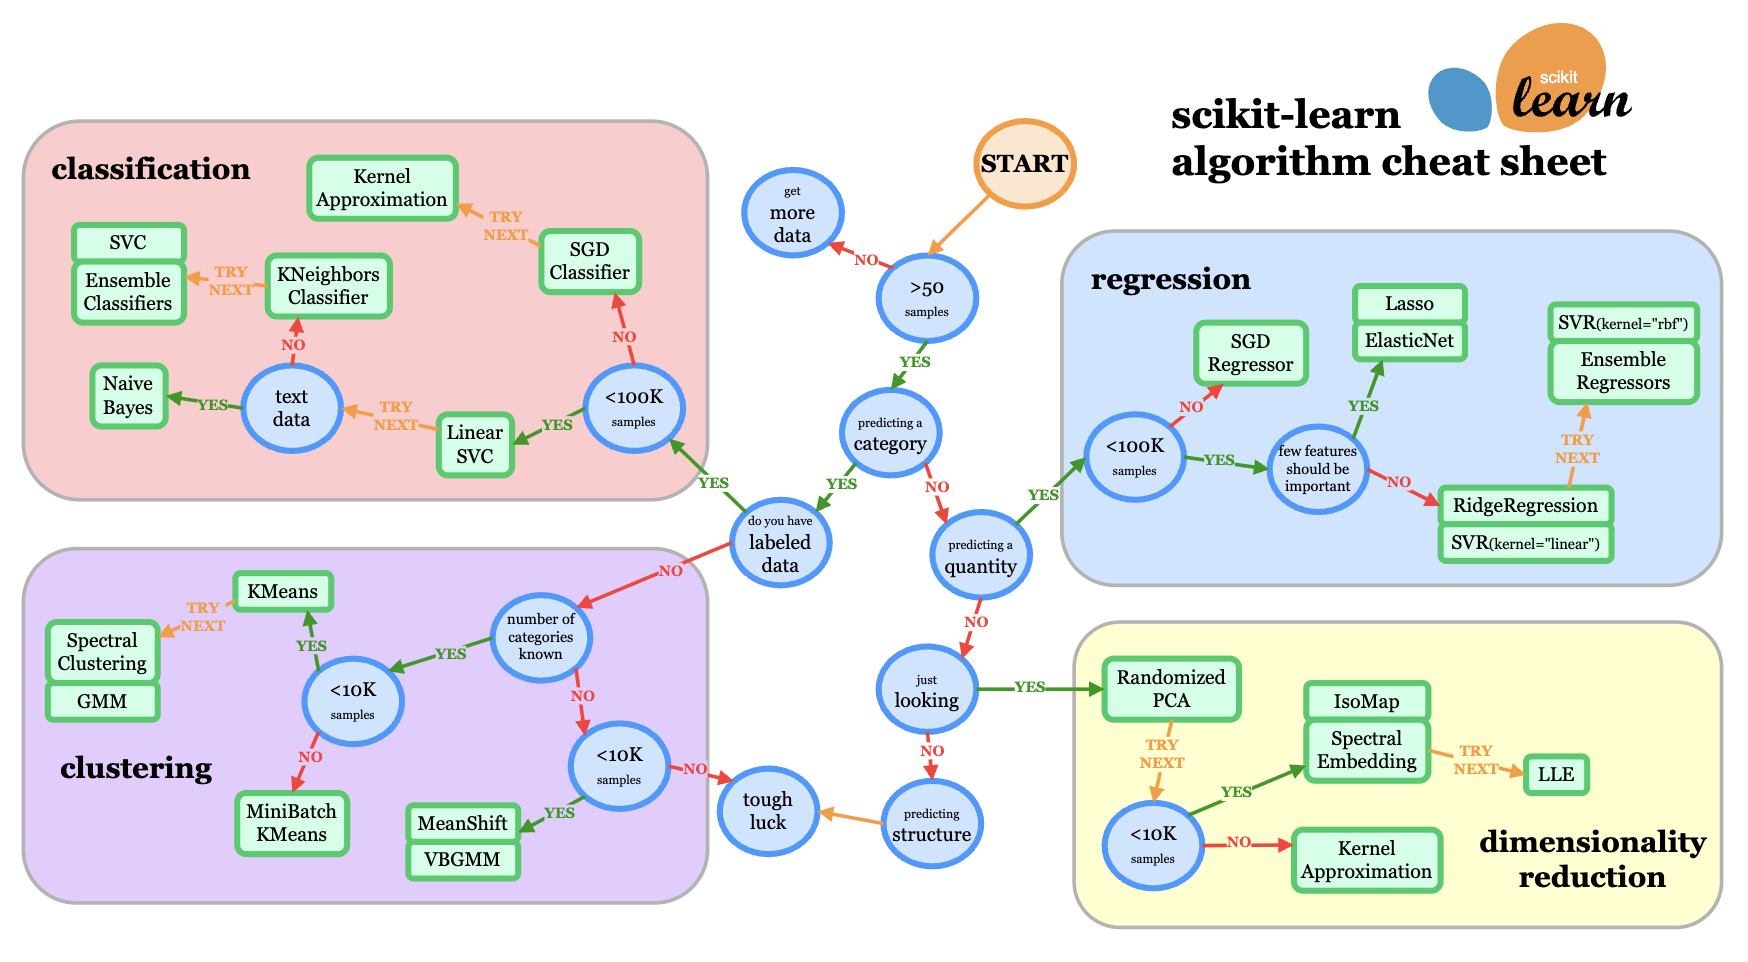
\includegraphics[width=0.9\linewidth]{algos.png}
\end{center}

Für unsere Iris nehmen wir aber einen Algorithmus, den wir bereits kennen: Den Entscheidungsbaum (oder \texttt{DecisionTreeClassifier()} innerhalb von \texttt{sklearn}).


\subsubsection*{Modell berechnen}


Wie eingangs erwähnt ist ein grosser Vorteil von \texttt{scikit learn}, dass verschiedene Algorithmen genau gleich verwendet werden können — obwohl sie sozusagen ``unter der Haube'' ganz anders funktionieren. Die Abstraktion macht den Umgang mit unterschiedlichen Algorithmen sehr angenehm und lädt auch zum Ausprobieren ein! Entscheidend ist hier die \texttt{.fit()}-Funktion, welche unabhängig vom ausgewählten Algorithmus die Berechnung des Modells vornimmt.

Die Funktion \texttt{fit()} ist in \texttt{scikit-learn} der Standardbefehl, um ein Modell zu trainieren. Der Name stammt aus dem Englischen und bedeutet in diesem Zusammenhang so viel wie \textit{anpassen}. Die Idee ist, dass das Modell versucht , möglichst gut zu den Trainingsdaten zu ``passen'' – es sucht ein mathematisches Modell, das den Zusammenhang zwischen den \texttt{features} (\texttt{X\_train}) und dem \texttt{target} (\texttt{y\_train}) beschreibt. Man sagt darum auch: \textit{``Das Modell wird an die Daten angepasst.''}

Im nachfolgenden Beispiel werden ein Entscheidungsbaum und ein KNN (ein Algorithmus, dessen Funktionsweise wir nicht behandelt haben) berechnet - beobachten Sie, wie klein der Unterschied hier ist!

\begin{lstlisting}[language=Python]
from scikit-learn import tree
classifier = tree.DecisionTreeClassifier() 
DT = classifier.fit(X_train,y_train)

from scikit-learn.neighbors import KNeighborsClassifier
classifier = KNeighborsClassifier(n_neighbors = 3) 
KNN = classifier.fit(X_train, y_train)
\end{lstlisting}

Wie Sie im Notizbuch sehen können, erlaubt Ihnen \texttt{sklearn} sogar, den automatisch berechneten Entscheidungsbaum darzustellen!

\subsection*{Evaluieren}
Wir können nun unser Modell \texttt{DT} (oder auch \texttt{KNN}) verwenden, um Vorhersagen zu treffen. Zunächst, bevor wir uns komplett neuen Irissen zuwenden, testen wir aber unser Modell anhand der Testdaten. Sollte sich herausstellen, dass unser Modell schon bei diesen Daten versagt, können wir nochmal über die Bücher. Wichtig ist zu verstehen, dass bei den Testdaten \textit{wir} wissen, was das Resultat sein soll, aber das Modell nicht. Das erlaubt uns überhaupt, zu überprüfen, ob das Modell richtig liegt oder nicht.

Hier ist das Iris-Beispiel sehr illustrativ: Wenn wir direkt, ohne diesen Evaluationsschritt ins Feld gehen, dann müssen wir — ausser Sie hätten eine entsprechende botanische Vorbildung — unserem Modell wohl oder übel glauben, da wir selbst nicht wissen, zu welcher Gattung eine bestimmte Iris gehört.

Die genauen Werte, die wir bei der Evaluation berechnen, sind ein Kapitel für sich; aber um eine Intuition zu bekommen, ob unser Modell eher gut oder schlecht ist, können wir Folgendes tun: Wir verwenden die Testdaten und vergleichen die Vorhersagen des Modells mit den tatsächlichen Werten (\texttt{y\_test}):

\begin{lstlisting}[language=Python]
y_pred = DT.predict(X_test)
\end{lstlisting}

Das Modell berechnet Vorhersagen (\texttt{y\_pred}) basierend auf den Test-\textit{features} \texttt{X\_test}. Diese vergleichen wir mit den echten Zielwerten \texttt{y\_test}.

Für eine erste Einschätzung genügt oft:

\begin{lstlisting}[language=Python]
DT.score(X_test, y_test)
\end{lstlisting}

Dieser Befehl gibt die \textbf{Genauigkeit} (\textit{accuracy}) zurück: den Anteil der Testbeispiele, bei denen das Modell die Klasse korrekt vorhergesagt hat.

Im Notizbuch wird dieser Schritt ganz am Ende durchgeführt, um es spannend zu machen. Dort sieht der Code etwas anders aus: Er zeigt für jede einzelne Zeile in \texttt{X\_test} was der entsprechende, richtige Wert in \texttt{y\_test} ist, und was das Modell vorhersagt.


\subsubsection*{Persistieren}
Auf diesem kleinen Datensatz geht das Berechnen ziemlich schnell voran — in der Wirklichkeit dauert aber das Berechnen eines Modells lange Zeit und nimmt viel Rechenleistung in Anspruch. Darum möchten wir die getane Arbeit auf keinen Fall wegwerfen und speichern (oder in Informatik-Sprache: \textit{persistieren}) unser Modell:

\begin{lstlisting}[language=Python]
import joblib
joblib.dump(DT, 'iris_tree.joblib')
\end{lstlisting}

Hierbei ist \texttt{DT} der Name unseres Modells, also das, was die \texttt{.fit()}-Funktion uns zurückgegeben hat. Mit dem folgenden Code können Sie das Modell später wieder laden - vorausgesetzt, dass Sie die Datei \texttt{iris\_tree.joblib} noch haben.

\begin{lstlisting}[language=Python]
DT = joblib.load('iris_tree.joblib')
\end{lstlisting}

\subsubsection*{Vorhersagen}
Nun sind wir endlich bereit, und wagen uns hinaus in die Natur mit unserem Modell. Wir stellen uns vor, dass wir als Belohnung für unsere Mühe zum berühmten Irisgarten des Meiji-Schreines in Tōkyō reisen, in welchem im Juni über 150 verschiedene Irisse blühen! 

\begin{figure}
\begin{center}
  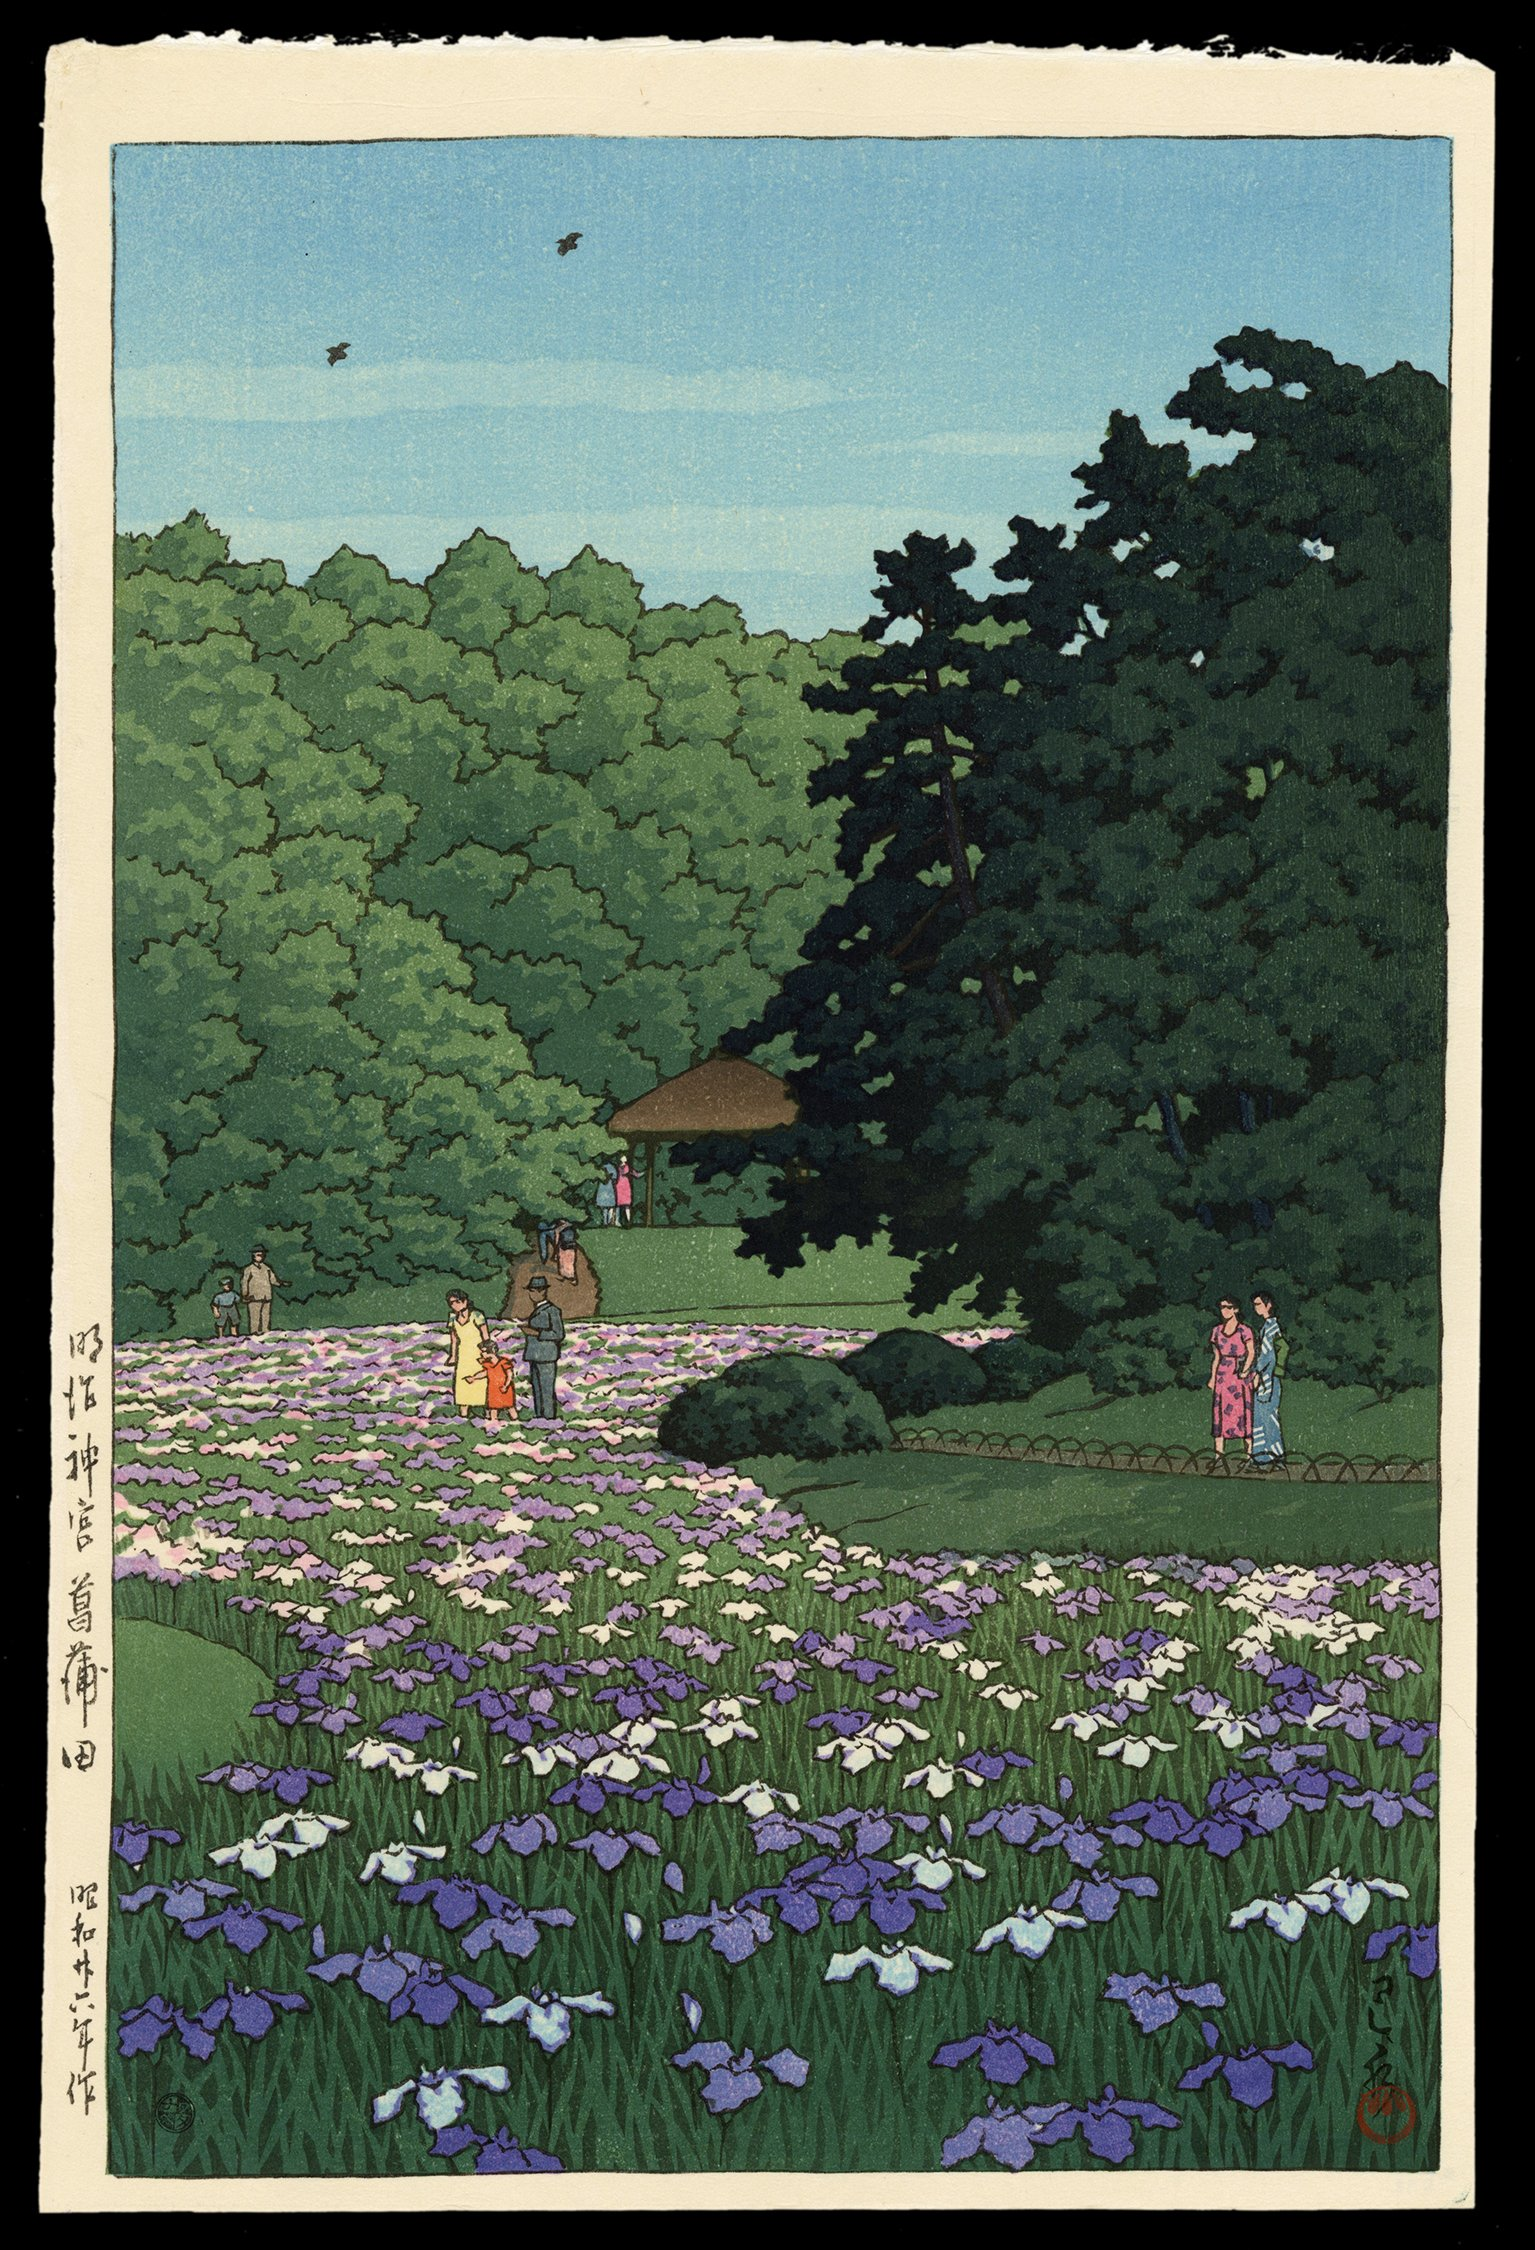
\includegraphics[width=0.5\linewidth]{irisgarden.jpg}
  \caption{Holzblock-Druck des Meiji-Schreines von Kawase Hasui (1883-1957)}
\end{center}
\end{figure}

Mit Erlaubnis der Behörden vermessen wir ein besonders hübsches Exemplar. Wir halten uns hier an die Reihenfolge der \textit{features} im Trainings-Datensatz:

\begin{lstlisting}[language=Python]
new_flower = [[5.1, 3.5, 12, 12]]
#              |    |    |   |
#              |    |    |   --- Länge des Blütenblatts in cm
#              |    |    ------- Breite des Blütenblatts in cm
#              |    ------------ Breite des Kelchblatts in cm
#              ----------------- Länge des Kelchblatts in cm
\end{lstlisting}

\begin{aufgabe}{3}
Diese Daten können wir aber nicht direkt so verwenden: Wir müssen alles, was wir mit den Trainingsdaten gemacht haben, auch mit den Daten für Vorhersagen machen. Was fehlt in diesem konkreten Fall noch?
\end{aufgabe}

Sobald wir die nötige Aufbereitung der Messdaten vorgenommen haben, können wir nun endlich unser Modell verwenden, um für komplett neue Daten eine Vorhersage zu treffen. In unserem Fall fragen wir unser Modell, zu welcher Iris-Art unser frisch vermessenes Exemplar zählt:

\begin{lstlisting}[language=Python]
DT.predict(new_flower_scaled)
\end{lstlisting}


\subsubsection*{Zusammenfassung}

In diesem Kapitel haben Sie gelernt, wie Sie mithilfe der Bibliothek \texttt{scikit-learn} maschinelles Lernen in Python praktisch umsetzen können. Anhand des bekannten Iris-Datensatzes haben Sie die typische Vorgehensweise kennengelernt:

\begin{itemize}
  \item \textbf{Importieren von Daten:} z. B. über \texttt{load\_iris(as\_frame=True)}
  \item \textbf{Zuweisung von \texttt{features} und \texttt{target}:} Eingabedaten (\texttt{X}) und Zielwerte (\texttt{y})
  \item \textbf{Aufteilen in Trainings- und Testdaten:} mit \texttt{train\_test\_split()}
  \item \textbf{Skalieren der Daten:} mit z.B. \texttt{MinMaxScaler()}
  \item \textbf{Modellwahl und Training:} mit \texttt{fit()}, z.B. \texttt{DecisionTreeClassifier()}
  \item \textbf{Evaluation des Modells:} mit \texttt{score()} oder Vergleich von \texttt{y\_test} und \texttt{y\_pred}
  \item \textbf{Modell speichern und laden:} mit \texttt{joblib.dump()} und \texttt{joblib.load()}
  \item \textbf{Vorhersagen treffen:} mit \texttt{predict()}
\end{itemize}

Die einheitliche Benennung (\texttt{fit()}, \texttt{predict()}, \texttt{score()}) erlaubt es, sehr einfach verschiedene ML-Algorithmen auszuprobieren ohne die gesamte Pipeline umstellen zu müssen. So können Sie Ihr Wissen über Entscheidungsbäume, lineare Regression oder \textit{k-means} direkt anwenden.





\end{lpu}



\subsection*{Didaktische Überlegungen}

In diesem Kapitel wurde bewusst auf eine grosse Anzahl entdeckender Aufgaben verzichtet. Der Grund dafür liegt in der Natur des behandelten Inhalts: Während viele frühere Kapitel dieser Unterrichtseinheit dazu einluden, Zusammenhänge und Strukturen selbständig zu entdecken (etwa bei Entscheidungsbäumen), handelt es sich hier um die praktische Umsetzung gelernter Konzepte in \texttt{python} und \texttt{scikit-learn}.

Die Umsetzung in Code ist in diesem Fall weniger ein Feld für offene Entdeckungen, sondern verlangt genaue Kenntnis spezifischer Befehle. Die APIs von \texttt{scikit-learn} sind zwar einheitlich und gut strukturiert, aber aufgrund des grossen Funktionsumfangs auch mit vielen möglichen Fehlerquellen verbunden. Selbst kleinere Unklarheiten bei den Argumenten einer Methode oder der Struktur der Eingabedaten führen schnell zu unverständlichen Fehlermeldungen oder nicht funktionierenden Vorhersagen.

Würde man die SuS in diesem Kapitel zu stark ``ausprobieren lassen'', wie es in konstruktivistisch geprägten Phasen sinnvoll ist, würde dies hier vor allem zu Frustration führen – insbesondere bei SuS, die noch nicht über viel Programmiererfahrung verfügen. Aus diesem Grund liegt der Fokus in diesem Abschnitt nicht auf Problemlösestrategien, sondern auf der \emph{sorgfältigen Übertragung Anwendung und Wiederholung} bereits erarbeiteter Inhalte. So kann Sicherheit im Umgang mit der Bibliothek aufgebaut werden, die sich später ausbauen liesse.


\subsection*{Musterlösungen}

\begin{aufgabe}{1}

Die Sitznachbarin hat sich entschieden, die alte Biologieprüfung auswendig zu lernen. Dabei hat sie sich nicht mit dem Stoff selbst, sondern mit dem \emph{genauen Wortlaut} der Aufgaben beschäftigt. Ihr Ziel war nicht, den Inhalt zu verstehen, sondern lediglich die exakten Fragen und Antworten zu memorieren.

Am Prüfungstag wurde sie jedoch überrascht: Die Lehrperson hat zwar ähnliche, aber nicht identische Fragen gestellt. Die zuvor auswendig gelernten Antworten helfen ihr jetzt kaum weiter. Wahrscheinlich wird sie Mühe haben, die neuen Fragen korrekt zu beantworten, weil sie den eigentlichen Stoff nie wirklich verstanden hat.

\textbf{Das ist ein klassisches Beispiel für \textit{overfitting}.} Im maschinellen Lernen bedeutet das, dass ein Modell die Trainingsdaten so gut ``gelernt'' hat, dass es nicht mehr auf neue, unbekannte Daten \textit{generalisieren} kann. Es hat nicht die \textit{Struktur} oder \textit{Logik} der Daten verstanden, sondern nur die Einzelbeispiele ``auswendig gelernt'' – wie die Schülerin die alte Prüfung.

\begin{itemize}
  \item \textbf{\textit{overfitting} anhand des Beispiels:}\\
  Die Sitznachbarin hat auswendig gelernt, statt zu verstehen. Das ist wie ein ML-Modell, das sich perfekt an die Trainingsdaten angepasst hat, aber bei neuen Daten versagt. Sie hat ein ``Modell'' erstellt, das nur für eine einzige Situation (die alte Prüfung) funktioniert. Sobald sich die Situation leicht ändert (neue Fragen), ist sie verloren.

  \item \textbf{Wie kann man \textit{overfitting} im ML vermeiden?}\\
  \begin{itemize}
    \item \textit{train-test split:} Man teilt die Daten in einen Trainings- und einen Testdatensatz. So kann überprüft werden, ob das Modell auch mit neuen Daten (Testdaten) gut funktioniert.
    \item \textit{Regulierung:} Manche Modelle erlauben Einstellungen, um extreme Anpassungen zu vermeiden (z.\,B. \texttt{max\_depth} bei Entscheidungsbäumen).
    \item \textit{Mehr Daten:} Wenn man viele unterschiedliche Trainingsbeispiele hat, ist es für das Modell schwieriger, ``auswendig zu lernen'' – und es lernt eher die allgemeinen Muster.
    \item \textit{cross validation:} Statt nur einmal zu testen, wird mehrfach mit unterschiedlichen Aufteilungen trainiert und getestet.
  \end{itemize}
\end{itemize}

\end{aufgabe}


\begin{aufgabe}{2}

\begin{enumerate}
  \item \textbf{\textit{one hot encoding} im Iris-Datensatz?}\\
  Im klassischen Iris-Datensatz ist das \texttt{y}-Array \textit{nicht} als \textit{one hot encoding} dargestellt, sondern als einfache Ganzzahlen:
  \begin{itemize}
    \item \texttt{0} steht für \textit{Iris setosa}
    \item \texttt{1} steht für \textit{Iris versicolor}
    \item \texttt{2} steht für \textit{Iris virginica}
  \end{itemize}
  Dies ist eine sogenannte \textit{integer encoded} Darstellung der Kategorien. Ein echtes \textit{one hot encoding} würde jede Kategorie mit einer einzigen 1 und sonst nur 0 dargestellt werden:
  \[
    \text{setosa} = [1, 0, 0],\quad
    \text{versicolor} = [0, 1, 0],\quad
    \text{virginica} = [0, 0, 1]
  \]

  \item \textbf{Sind die \texttt{X}-Werte im gleichen Wertebereich?}\\
  Nein. Die vier Spalten von \texttt{X} enthalten:
  \begin{itemize}
    \item \texttt{sepal length (cm)} – z. B. Werte um 5–7
    \item \texttt{sepal width (cm)} – z. B. 2–4
    \item \texttt{petal length (cm)} – z. B. 1–6.5
    \item \texttt{petal width (cm)} – z. B. 0.1–2.5
  \end{itemize}
  Die Werte liegen also in unterschiedlichen Bereichen und Skalen. Einige Spalten enthalten kleine Werte (z. B. \texttt{petal width}), andere deutlich grössere (\texttt{petal length}). Das könnte Algorithmen beeinflussen, die diese numerische Abstände berücksichtigen. Eine Skalierung (z. B. mit \texttt{MinMaxScaler} oder \texttt{StandardScaler}) könnte hier sinnvoll sein, um alle \textit{features} in denselben Bereich zu bringen und die Algorithmen nicht zu verzerren.
\end{enumerate}

\end{aufgabe}


\begin{aufgabe}{3}

Die neuen Daten (also neue Messungen der Blume) liegen im Rohformat vor – das heisst: Sie sind noch \textit{nicht skaliert}.

Da unser Modell jedoch mit skaliertem \texttt{X\_train} trainiert wurde, ist ein direkter Vergleich nicht möglich. Das Modell erwartet Eingabewerte im Bereich von $0$ bis $1$, nicht in Zentimetern. Wir müssen also auch die neuen Daten zuerst durch den \texttt{Scaler} schicken, mit dem wir die Trainingsdaten skaliert haben:

\begin{lstlisting}[language=Python]
new_flower_scaled = scaler.transform(new_flower)
\end{lstlisting}

Erst danach dürfen wir sie für eine Vorhersage verwenden:

\begin{lstlisting}[language=Python]
prediction = model.predict(new_flower_scaled)
\end{lstlisting}

Bei neuen Eingabedaten müssen immer dieselben \textit{preprocessing}-Schritte durchgeführt werden wie bei den Trainingsdaten – sonst ``versteht'' das Modell die Zahlen nicht im richtigen Kontext.

\end{aufgabe}
